\documentclass[12pt,hyperref,a4paper,UTF8]{ctexart}
\usepackage{HDUReport}
\usepackage{listings}
\usepackage{xcolor}
\usepackage{graphicx}
\usepackage{setspace}
\usepackage{float}
\setstretch{1.5} % 设置全局行距为1.5倍

\usepackage{enumitem} % 载入enumitem包以便自定义列表环境
\setlist[itemize]{itemsep=0pt, parsep=0pt} % 设置itemize环境的项目间距和段落间距

\setmainfont{Times New Roman} % 英文正文为Times New Roman


\usepackage{tikz}
\usetikzlibrary{shapes.geometric, arrows}
\usetikzlibrary{positioning, arrows.meta}
\usetikzlibrary{calc}


% 设置MATLAB代码样式
\definecolor{codegreen}{rgb}{0,0.6,0}
\definecolor{codegray}{rgb}{0.5,0.5,0.5}
\definecolor{codepurple}{rgb}{0.58,0,0.82}
\definecolor{backcolour}{rgb}{0.95,0.95,0.92}

\lstdefinestyle{matlab}{
    backgroundcolor=\color{backcolour},   
    commentstyle=\color{codegreen},
    keywordstyle=\color{magenta},
    numberstyle=\tiny\color{codegray},
    stringstyle=\color{codepurple},
    basicstyle=\ttfamily\small,
    breakatwhitespace=false,         
    breaklines=true,                 
    captionpos=b,                    
    keepspaces=true,                 
    numbers=left,                    
    numbersep=5pt,                  
    showspaces=false,                
    showstringspaces=false,
    showtabs=false,                  
    tabsize=2,
    frame=single,
    language=Matlab
}
%封面页设置
{   
    %标题
    \title{ 
        \vspace{1cm}
        \heiti \Huge \textbf{《数字信号处理课程设计》实验报告} \par
        \vspace{1cm} 
        \heiti \Large {\underline{实验报告1:线性卷积与圆周卷积的计算/利用FFT实现线性卷积}   } 
        \vspace{3cm}
    
    }

    \author{
        \vspace{0.5cm}
        \kaishu\Large 学院\ \dlmu[9cm]{卓越学院} \\ %学院
        \vspace{0.5cm}
        \kaishu\Large 学号\ \dlmu[9cm]{23040447} \\ %班级
        \vspace{0.5cm}
        \kaishu\Large 姓名\ \dlmu[9cm]{陈文轩} \qquad  \\ %学号
        \vspace{0.5cm}
        \kaishu\Large 专业\ \dlmu[9cm]{智能硬件与系统(电子信息工程)} \qquad \\ %姓名 
    }
        
    \date{\today} % 默认为今天的日期,可以注释掉不显示日期
}
%%------------------------document环境开始------------------------%%
\begin{document}

%%-----------------------封面--------------------%%
\cover
\thispagestyle{empty} % 首页不显示页码
%%------------------摘要-------------%%
%\newpage
%\begin{abstract}




%\end{abstract}

%\thispagestyle{empty} % 首页不显示页码

%%--------------------------目录页------------------------%%
% \newpage
% \tableofcontents
% \thispagestyle{empty} % 目录不显示页码

%%------------------------正文页从这里开始-------------------%
\newpage
\setcounter{page}{1} % 让页码从正文开始编号

%%可选择这里也放一个标题
%\begin{center}
%    \title{ \Huge \textbf{{标题}}}
%\end{center}
\section{实验目的}
1、掌握计算机的使用方法和常用系统软件及应用软件的使用;

2、通过MATLAB编程,上机调试程序,进一步增强使用计算机解决问题的能力;

3、通过实验一,掌握线性卷积与循环卷积软件实现的方法,并验证二者之间的关系;

4、通过实验三,加深理解 FFT在实现数字滤波(或快速卷积)中的重要作用,更好的利用 FFT进行数字信号处理。

5、进一步掌握循环卷积和线性卷积两者之间的关系。


\section{实验基本原理}
\subsection{实验一:线性卷积与圆周卷积的计算}

线性卷积和圆周卷积是数字信号处理中两种基本的序列运算方式,在信号分析、滤波器设计及频谱分析中有广泛应用。

\subsubsection{线性卷积}
对于长度为$N_1$的序列$x[n]$和长度为$N_2$的序列$h[n]$,两者的线性卷积定义为:
\begin{equation}
y[n] = x[n] * h[n] = \sum_{m=0}^{N_2-1} h[m]x[n-m]
\end{equation}

线性卷积的结果序列长度为$N_1+N_2-1$。在本实验中,我们使用MATLAB内置函数\texttt{conv()}计算序列$x$和$h$的线性卷积。

\subsubsection{圆周卷积}
圆周卷积(循环卷积)是在周期延拓的基础上进行的卷积运算。对于长度为$N$的序列$x[n]$和$h[n]$,其圆周卷积定义为:
\begin{equation}
y[n] = x[n] \circledast h[n] = \sum_{m=0}^{N-1} h[m]x[(n-m)_N]
\end{equation}
其中,$(n-m)_N$表示取模运算,即$(n-m) \mod N$。

圆周卷积的结果序列长度与运算周期$N$相同。在本实验中,我们通过自定义函数\texttt{circonv()}计算不同长度($N=5,6,9,10$)的圆周卷积。

\subsection{实验三:利用FFT实现线性卷积}

快速傅里叶变换(FFT)是离散傅里叶变换(DFT)的高效计算算法,可以显著降低计算复杂度,从$O(N^2)$降至$O(N\log N)$。利用FFT实现线性卷积是数字信号处理中的重要应用,尤其对于长序列的卷积计算具有明显优势。

\subsubsection{卷积定理}
根据卷积定理,两个序列的线性卷积等价于它们傅里叶变换的乘积的逆变换:
\begin{equation}
y[n] = x[n] * h[n] \Leftrightarrow Y(k) = X(k) \cdot H(k)
\end{equation}

其中$X(k)$和$H(k)$分别是序列$x[n]$和$h[n]$的离散傅里叶变换,$Y(k)$是它们的频域乘积。

\subsubsection{FFT实现线性卷积的步骤}
对于长度为$N_1$的序列$x[n]$和长度为$N_2$的序列$h[n]$,利用FFT实现线性卷积的基本步骤如下:

\begin{enumerate}
    \item 确定变换长度$N \geq N_1 + N_2 - 1$,通常选择$N = N_1 + N_2 - 1$
    \item 对序列$x[n]$和$h[n]$进行零填充,使其长度达到$N$
    \item 计算零填充后序列的FFT:$X(k) = \text{FFT}(x[n], N)$,$H(k) = \text{FFT}(h[n], N)$
    \item 计算频域乘积:$Y(k) = X(k) \cdot H(k)$
    \item 计算逆FFT得到线性卷积结果:$y[n] = \text{IFFT}(Y(k), N)$
\end{enumerate}

\subsubsection{本实验原理}
在本实验中,我们利用FFT实现了数字滤波器对不同输入信号的滤波过程,本质上是计算输入信号与滤波器脉冲响应的线性卷积。实验中:

\begin{itemize}
    \item 数字滤波器脉冲响应序列$h[n] = 0.5^n$,为指数衰减序列,长度为$N_1$
    \item 三种输入序列:
    \begin{itemize}
        \item $x_1[n]$为单位阶跃序列,全为1
        \item $x_2[n]$为余弦序列,$x_2[n] = \cos(2\pi n/N_2)$
        \item $x_3[n]$为指数衰减序列,$x_3[n] = 0.33^n$
    \end{itemize}
    \item 确定变换长度$N = N_1 + N_2 - 1$
    \item 对输入序列和滤波器脉冲响应计算FFT
    \item 在频域相乘实现滤波:$Y_i(k) = X_i(k) \cdot H(k)$,其中$i = 1,2,3$
    \item 通过IFFT得到时域滤波结果$y_i[n]$
\end{itemize}


FFT实现线性卷积的方法在实际应用中被广泛用于数字滤波器设计、系统辨识、语音处理和图像处理等领域。



\section{实验要求及内容}

\subsection{实验一}


已知两个有限长序列
\begin{align*}
x(n) &= \delta(n) + 2\delta(n-1) + 3\delta(n-2) + 4\delta(n-3) + 5\delta(n-4) \\
h(n) &= \delta(n) + 2\delta(n-1) + \delta(n-2) + 2\delta(n-3)
\end{align*}
\begin{enumerate}
    \item 实验前,预先预算好这两个序列的线性卷积及N=5,6,9,10循环卷积:
    \item 将实验结果与预先笔算的结果比较,验证其正确性。
\end{enumerate}

笔算过程与结果如下:


\begin{figure}[H] % [H] 表示强制当前位置插入
        \centering
        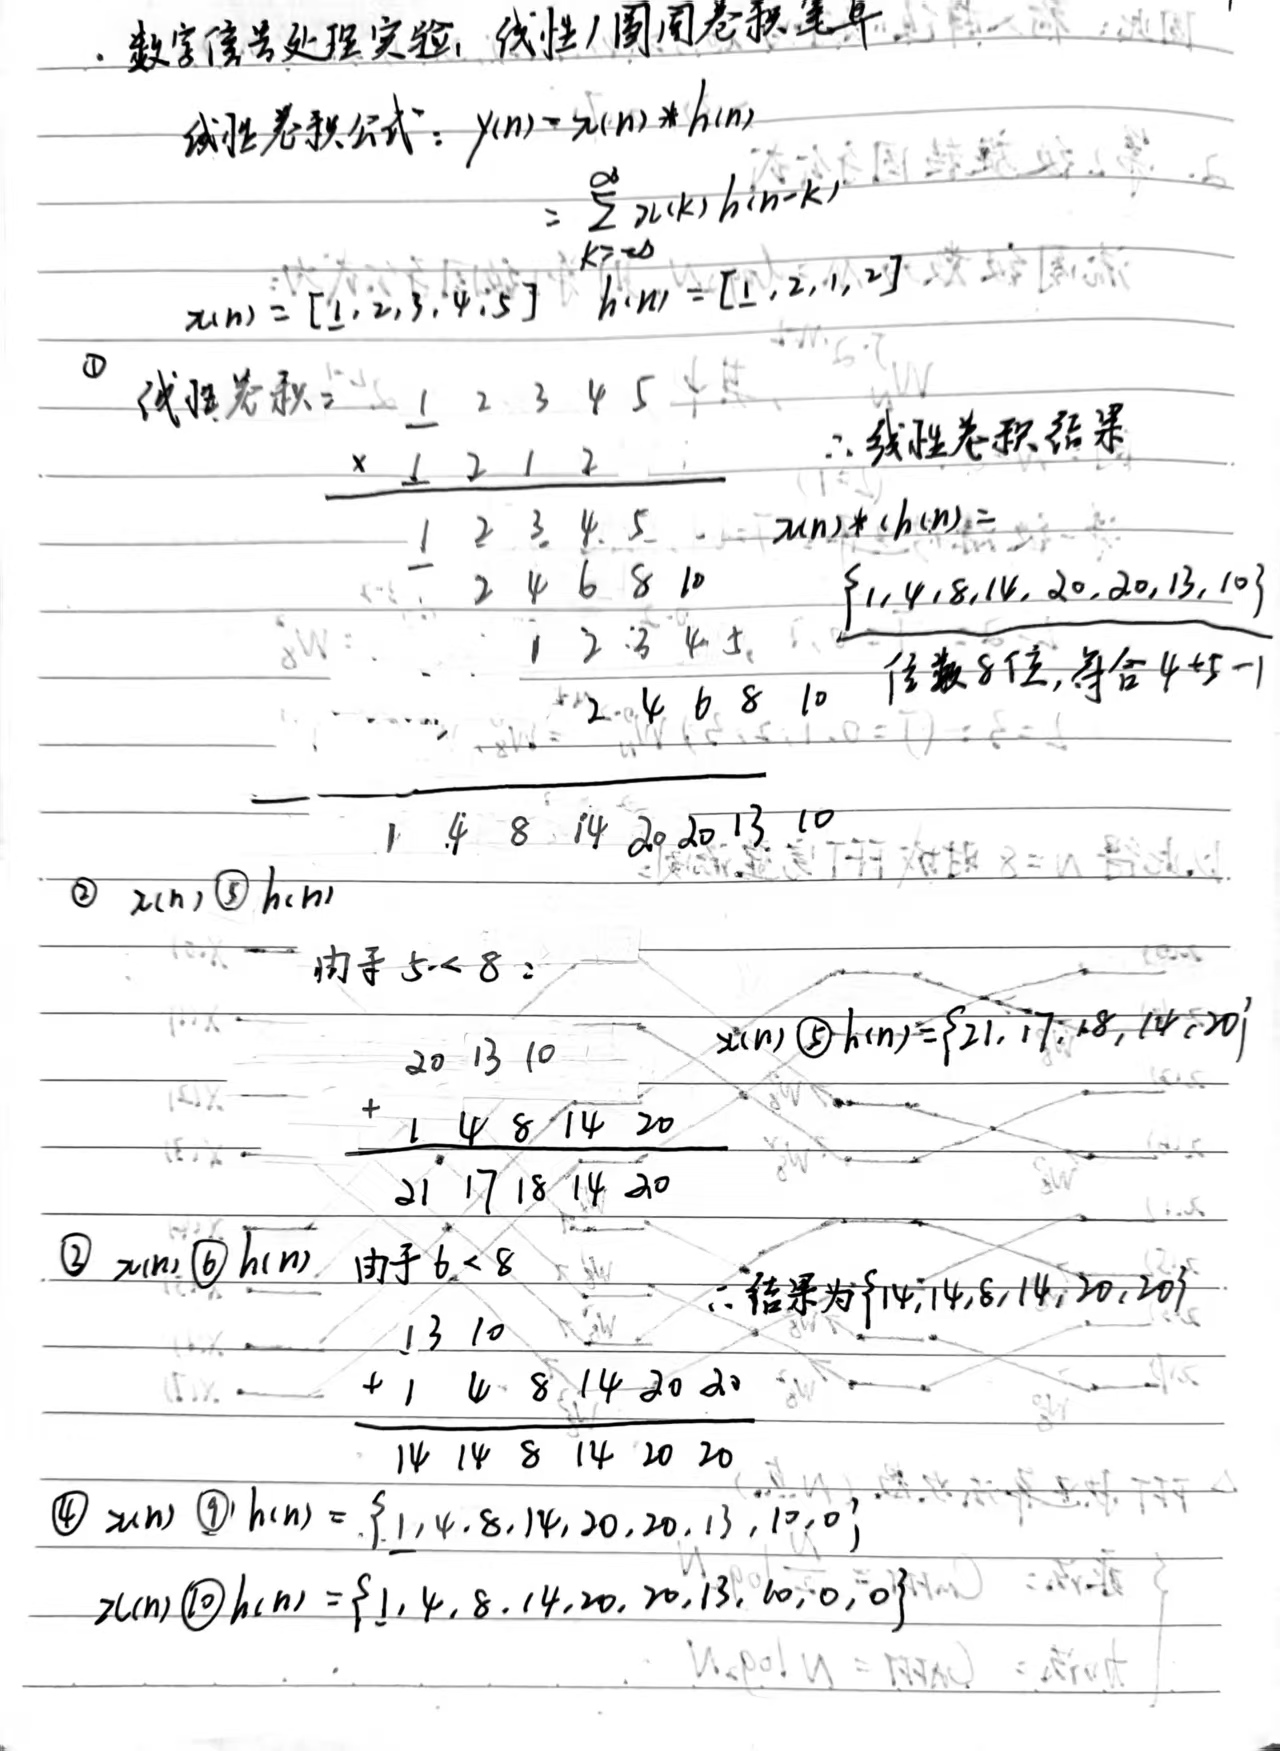
\includegraphics[width=1\textwidth]{figures/201.jpg} % 调整宽度为文本宽度的 80%
        \caption{笔算结果} %图片标题
        \label{fig:example} % 图片标签,用于引用
\end{figure}

\subsection{实验三}

数字滤波器的脉冲响应为 \(h(n) = (\frac{1}{2})^n R_{N2}(n), N_2\) 可自定,本实验取 \(N_2 = 17\)

输入序列 \(x(n)\) 可选下列几种情况
\begin{align*}
\textcircled{1} \, \text{x}(n) &= R_{N1}(n) \qquad N_1 \text{ 可取 } 16 \\
\textcircled{2} \, \text{x}(n) &= \cos(\frac{2\pi}{N_1} n) R_{N1}(n) \quad N_1 = 16 \\
\textcircled{3} \, \text{x}(n) &= (\frac{1}{3})^n R_{N1}(n), \quad N_1 = 16
\end{align*}
2、实验前,预先计算好 \(x(n) * h(n)\) 的值。



\section{实验结果与分析}

\subsection{实验一}

\subsubsection{代码实现}
% 插入MATLAB代码
\begin{lstlisting}[style=matlab, caption={实验一MATLAB实现代码}]
% 主函数
clear all;
n = 0:1:11;
m = 0:1:5;
N1 = length(n);
N2 = length(m);
x = [1 2 3 4 5]; %定义序列x
h = [1 2 1 2]; %定义序列h
res_conv = conv(x,h); % 计算线性卷积
res_circonv5 = circonv(x,h,5);% 计算圆周卷积
res_circonv6 = circonv(x,h,6) ; % 计算圆周卷积
res_circonv9 = circonv(x,h,9); % 计算圆周卷积
res_circonv10 = circonv(x,h,10); % 计算圆周卷积
ny1 = 0:length(res_conv)-1;  % 定义线性卷积的输出时域
ny2 = 0:length(res_circonv5)-1; % 定义圆周卷积的输出时域
ny3 = 0:length(res_circonv6)-1;
ny4 = 0:length(res_circonv9)-1;
ny5 = 0:length(res_circonv10)-1;
subplot(5, 1, 1);
stem(ny1, res_conv);  % 绘制线性卷积结果
subplot(5, 1, 2);
stem(ny2, res_circonv5);  % 绘制圆周卷积结果
subplot(5, 1, 3);
stem(ny3, res_circonv6); 
subplot(5, 1, 4);
stem(ny4, res_circonv9); 
subplot(5, 1, 5);
stem(ny5, res_circonv10); 
axis([0, 10, 0, 25]);  % 设置坐标轴范围
\end{lstlisting}
\subsubsection{效果展示}


\begin{figure}[H] % [H] 表示强制当前位置插入
        \centering
        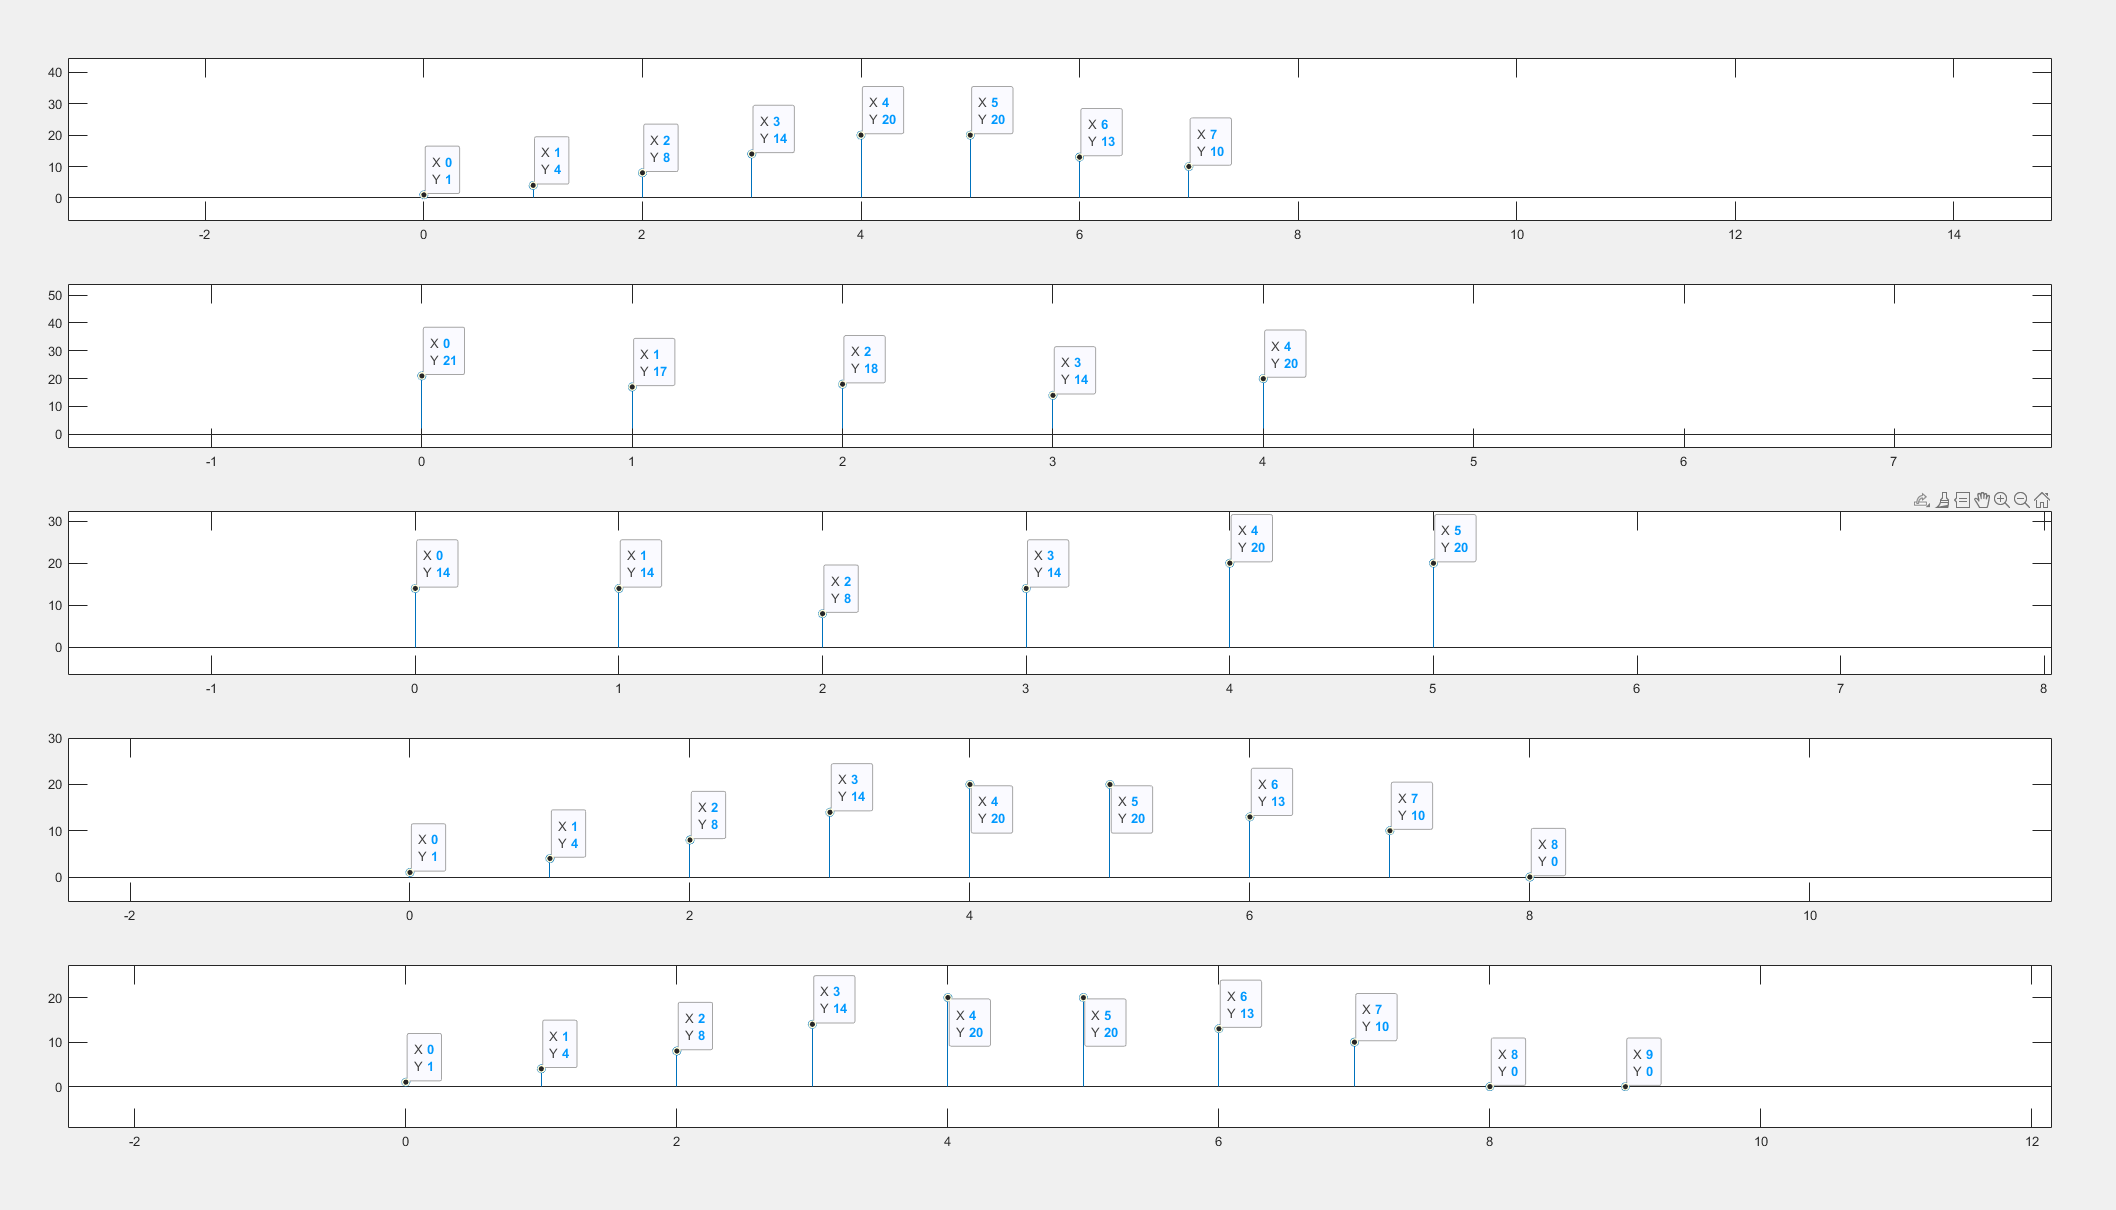
\includegraphics[width=0.9\textwidth]{figures/301.png} % 调整宽度为文本宽度的 80%
        \caption{matlab绘图} %图片标题
        \label{fig:example} % 图片标签,用于引用
\end{figure}



\subsection{实验三}

\subsubsection{代码实现}
% 插入MATLAB代码
\begin{lstlisting}[style=matlab, caption={实验三MATLAB实现代码}]
n= [0:1:17];
m= [0:1:16];
Nl=length(n);
N2=length(m);
hn=0.5.^n;  %生成数字滤波器脉冲序列 hn为0.5指数衰减序列
x1n=ones(1,N2); %生成输入序列x1n 即 x1[n]=[1,1,1,...,1](单位步进序列)
x2n=ones(1,N2).*cos(2*pi/N2*m); %生成一个余弦波序列x2n = cos(2πn/N2)
x3n=ones(1,N2).*0.33.^m; %生成一个指数衰减序列 x3[n]= 0.33^n
N=N1+N2-1;
X1K=fft(x1n, N); %输入序列和数字滤波器脉冲序列进行FFT运算
X2K=fft(x2n, N);
X3K=fft(x3n, N);
HK=fft(hn, N);
Y1K=X1K.*HK;   %频域相乘=时域卷积 FFT数字滤波实现关键 Xi[n]此时滤波
Y2K=X2K.*HK;
Y3K=X3K.*HK;
y1n=ifft(Y1K,N); %反傅里叶变换 由频域得到时域结果
y2n=ifft(Y2K,N);
y3n=ifft(Y3K,N);
x=0:N-1;
subplot(3, 1, 1);%将计算结果呈现在图表上
stem(x,y1n,'.');
subplot(3, 1, 2);
stem(x,y2n,'.');
subplot(3, 1 , 3);
stem(x,y3n,'.');
\end{lstlisting}
\subsubsection{效果展示}


\begin{figure}[H] % [H] 表示强制当前位置插入
        \centering
        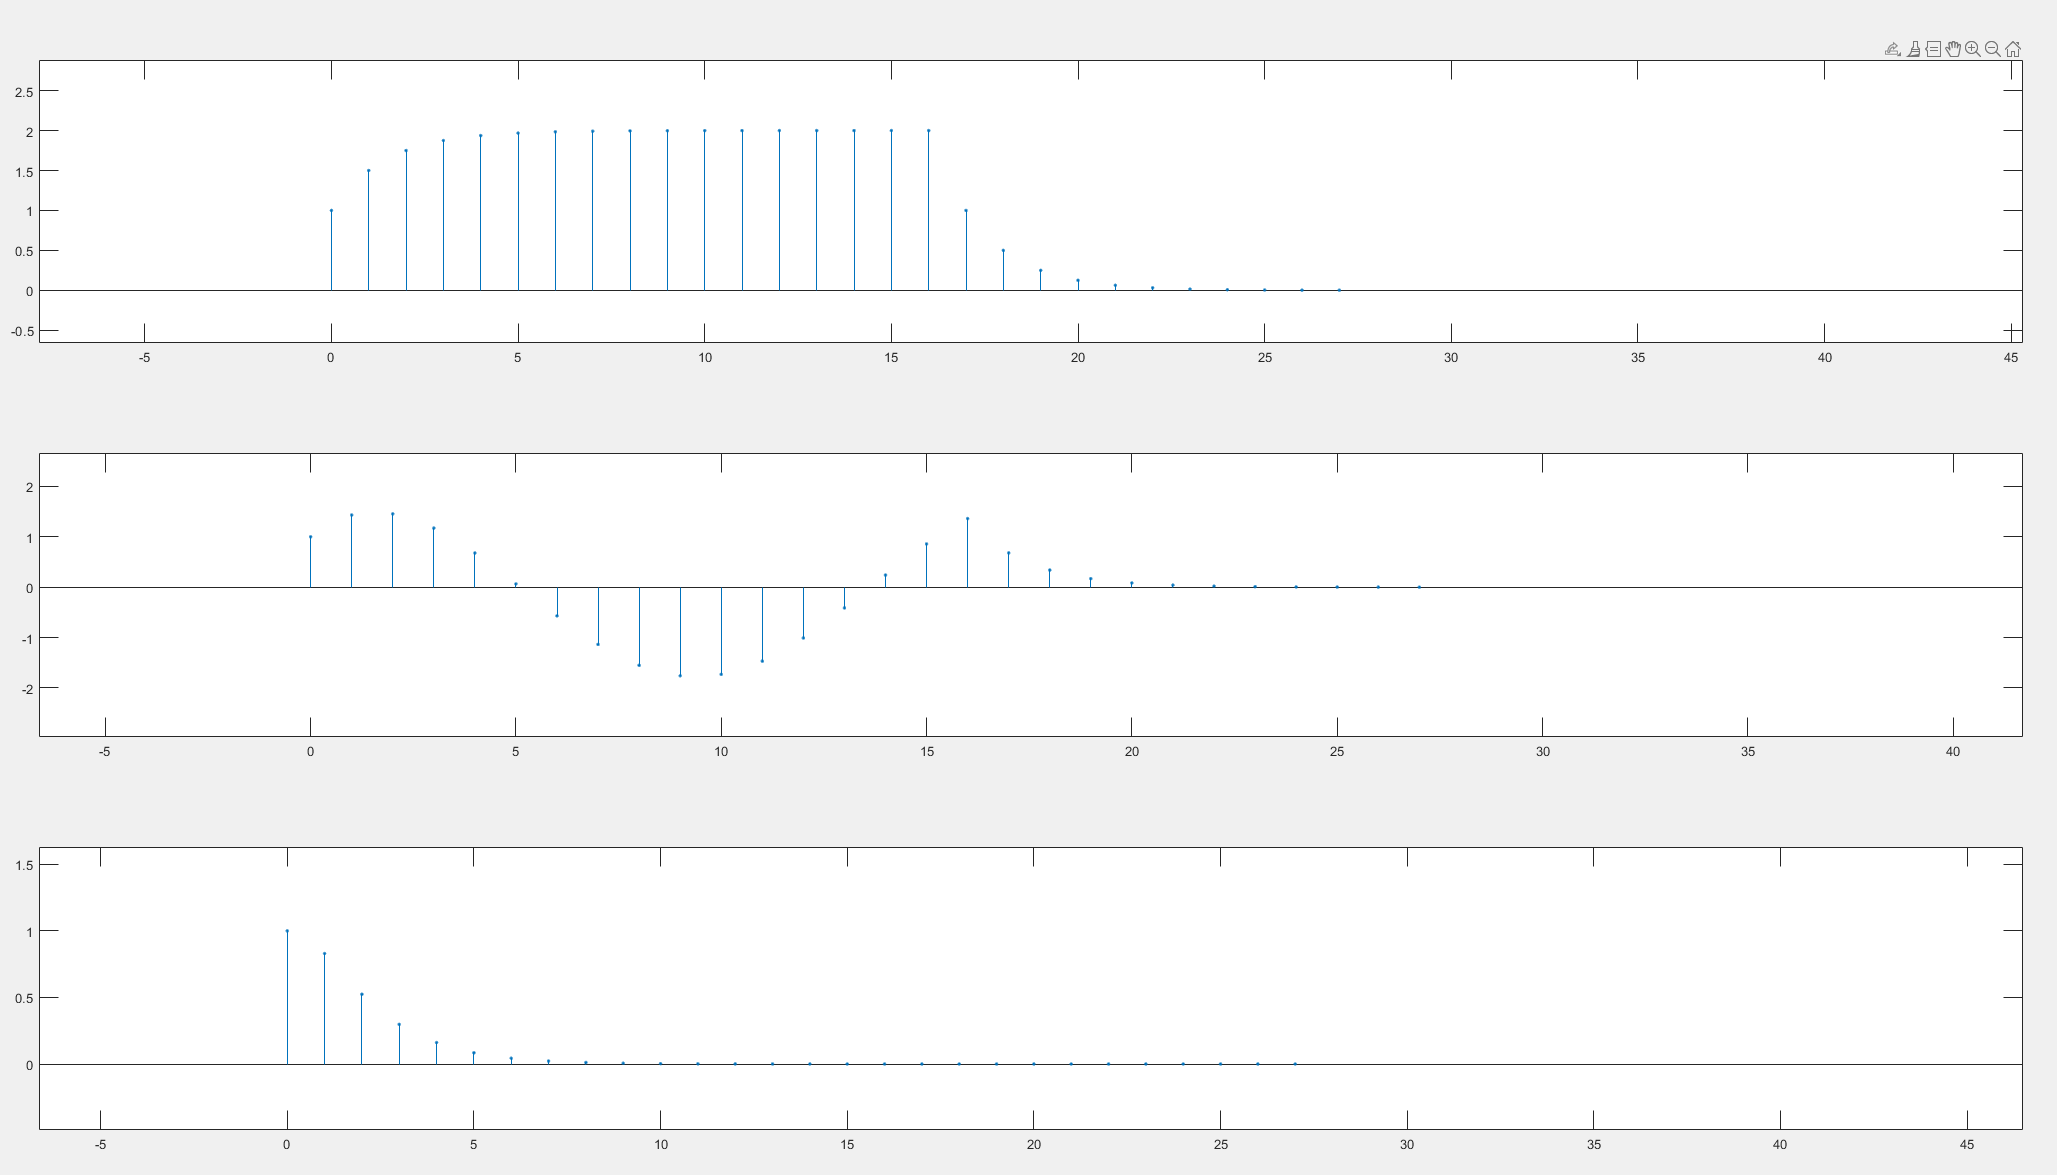
\includegraphics[width=0.9\textwidth]{figures/302.png} % 调整宽度为文本宽度的 80%
        \caption{matlab绘图} %图片标题
        \label{fig:example} % 图片标签,用于引用
\end{figure}

\section{实验小结}
本次实验主要完成了两个任务:线性卷积与圆周卷积的计算,以及利用FFT实现线性卷积。通过MATLAB编程,我们实现了两个序列的线性卷积和不同长度(N=5,6,9,10)下的圆周卷积计算,验证了当圆周卷积长度N≥N₁+N₂-1时与线性卷积结果相同的理论。同时,我们也利用FFT算法实现了数字滤波器对三种不同输入信号(单位阶跃序列、余弦序列和指数衰减序列)的滤波过程,验证了卷积定理在实际应用中的有效性。实验加深了对卷积运算和FFT在数字信号处理中应用的理解,掌握了频域方法提高计算效率的重要技术。




\end{document}